\begin{figure}[!ht]
	\begin{center}
		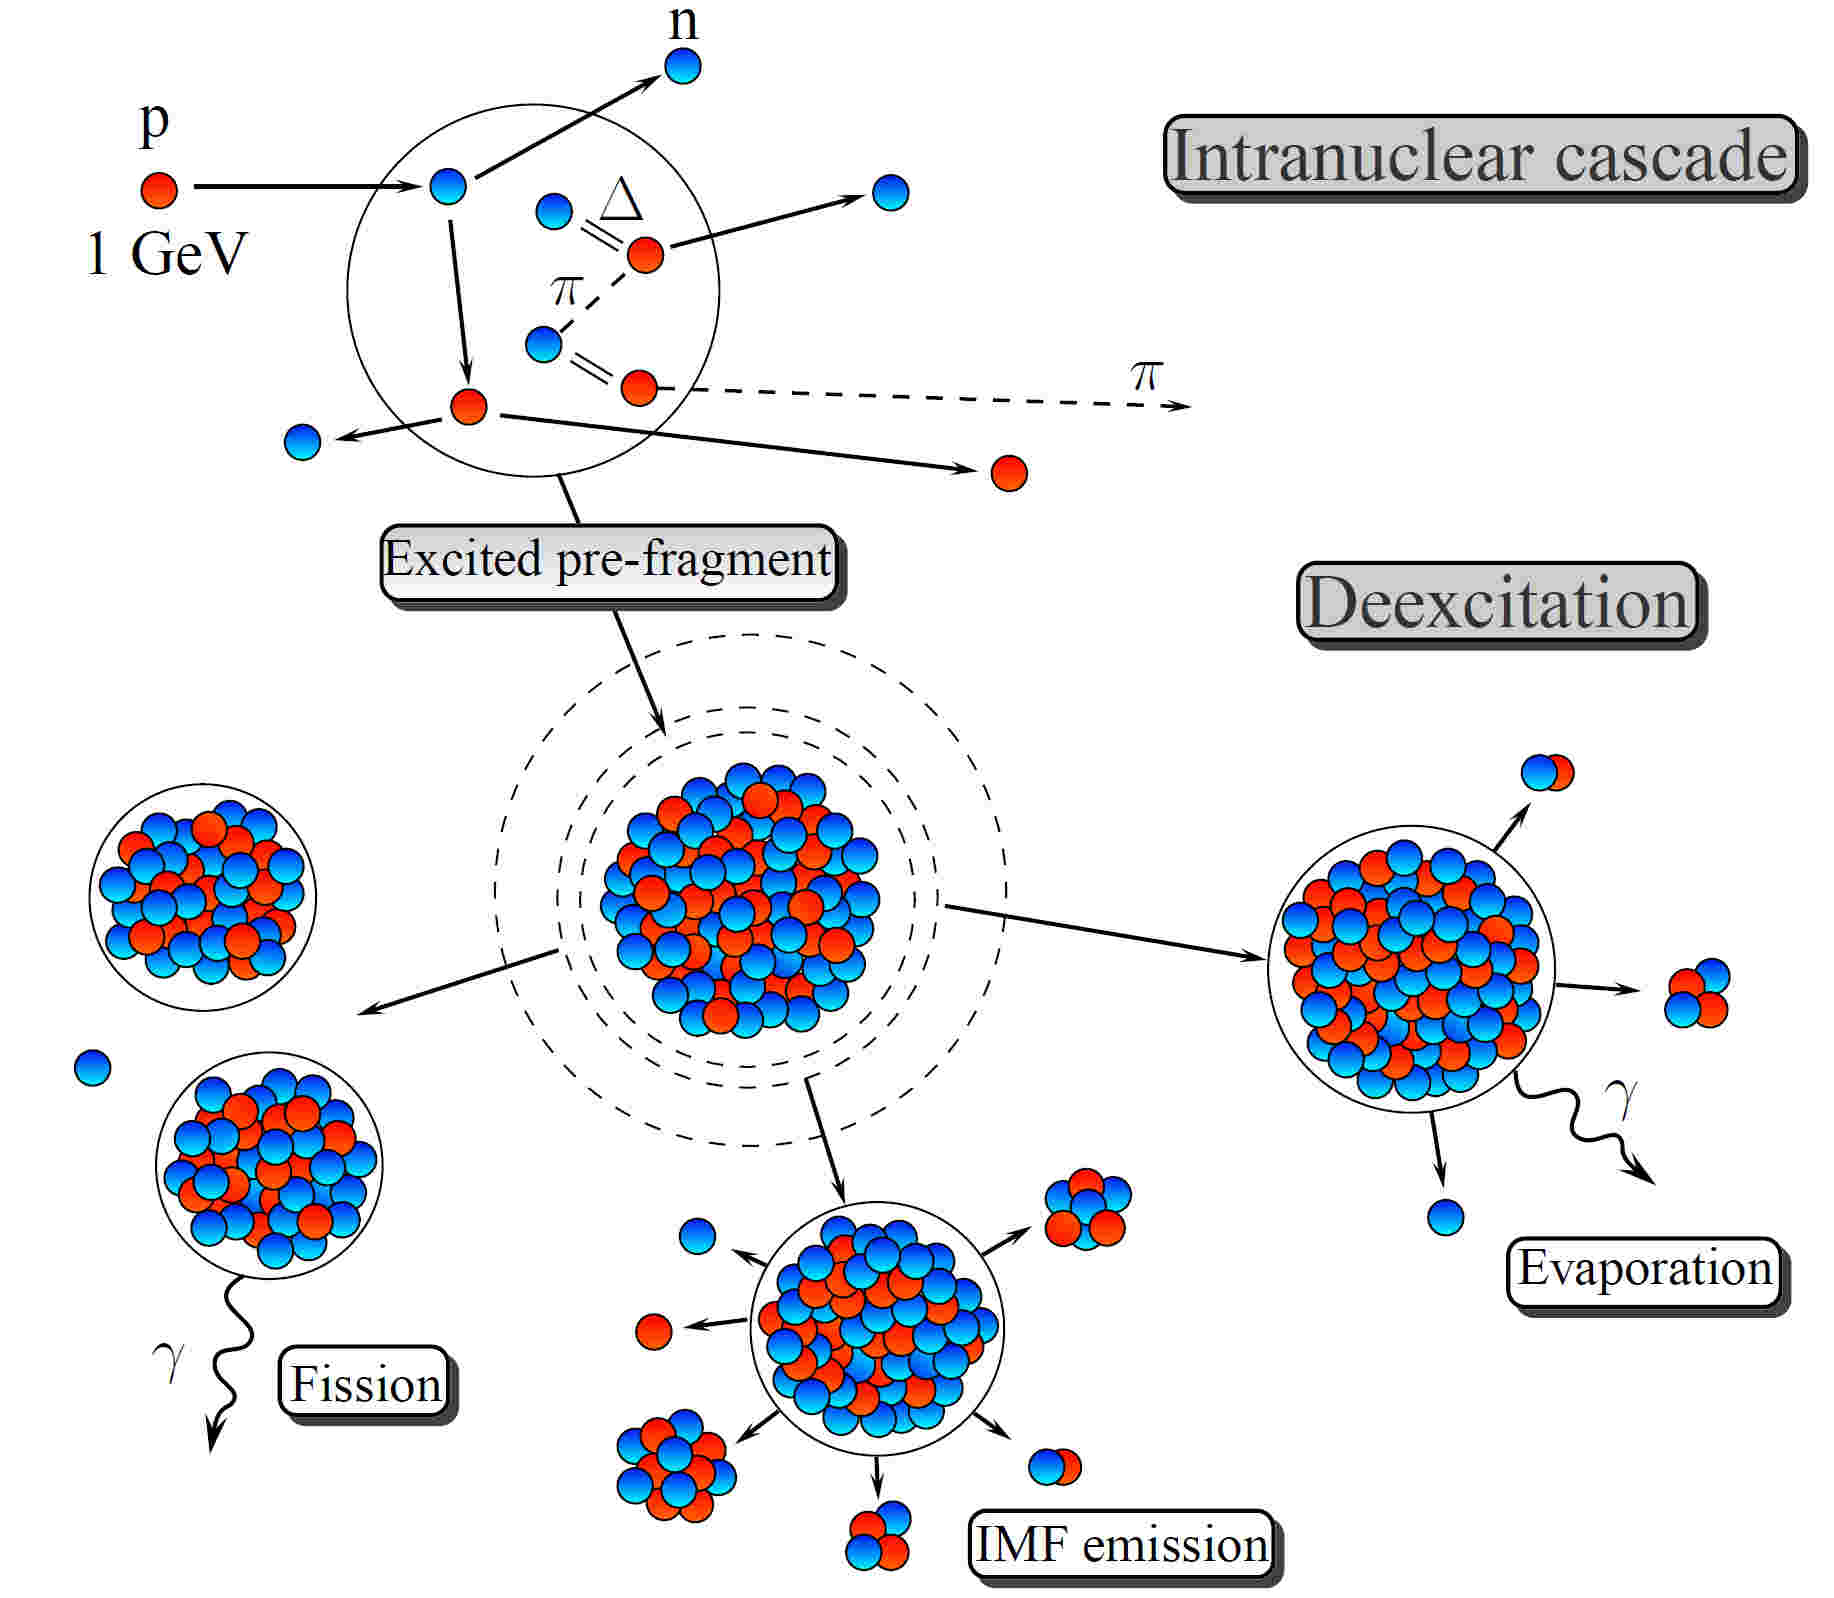
\includegraphics[width=\textwidth]{01_Introduction/figures/fig000_spallation}
	\end{center}
	\caption[Schematic view of the spallation process.]{Schematic view of the spallation process \cite{gorbinet:tel-00660583}. The incident proton interact with nucleons of the target nucleus. An intranuclear cascade occurs leaving the target atom in a excited state. Depending of property of the excited nucleus, different de-excitation process may occur.}
	\label{chap1:fig:spallation}
\end{figure}
